\level{2}{Applicazione Android}
    Dopo che in precedenza è stata fornita una descrizione generale dell'Applicazione Android, è qui riportata la sua progettazione architetturale.\\
    La presente sezione riporta i risultati ottenuti tramite una rigida struttura:
    \begin{enumerate}
        \item vengono presentate e successivamente descritte le componenti individuate;
        \item vengono descritte le interazioni che possono avvenire tra le componenti che sono state individuate;
        \item vengono descritti e contestualizzati gli eventuali design pattern che sono stati utilizzati durante la progettazione delle componenti;
        \item vengono descritte le classi che sono state individuate all'interno di ciascuna componente (eventualmente suddivise per package di appartenenza);
        \item vengono descritte le interazioni tra le classi che sono state individuate;
        \item vengono descritti e contestualizzati i design pattern che sono stati utilizzati durante la progettazione delle classi.
    \end{enumerate}
	
    \level{3}{Descrizione delle componenti dell'Applicazione}
        \begin{figure}[H]\centering
            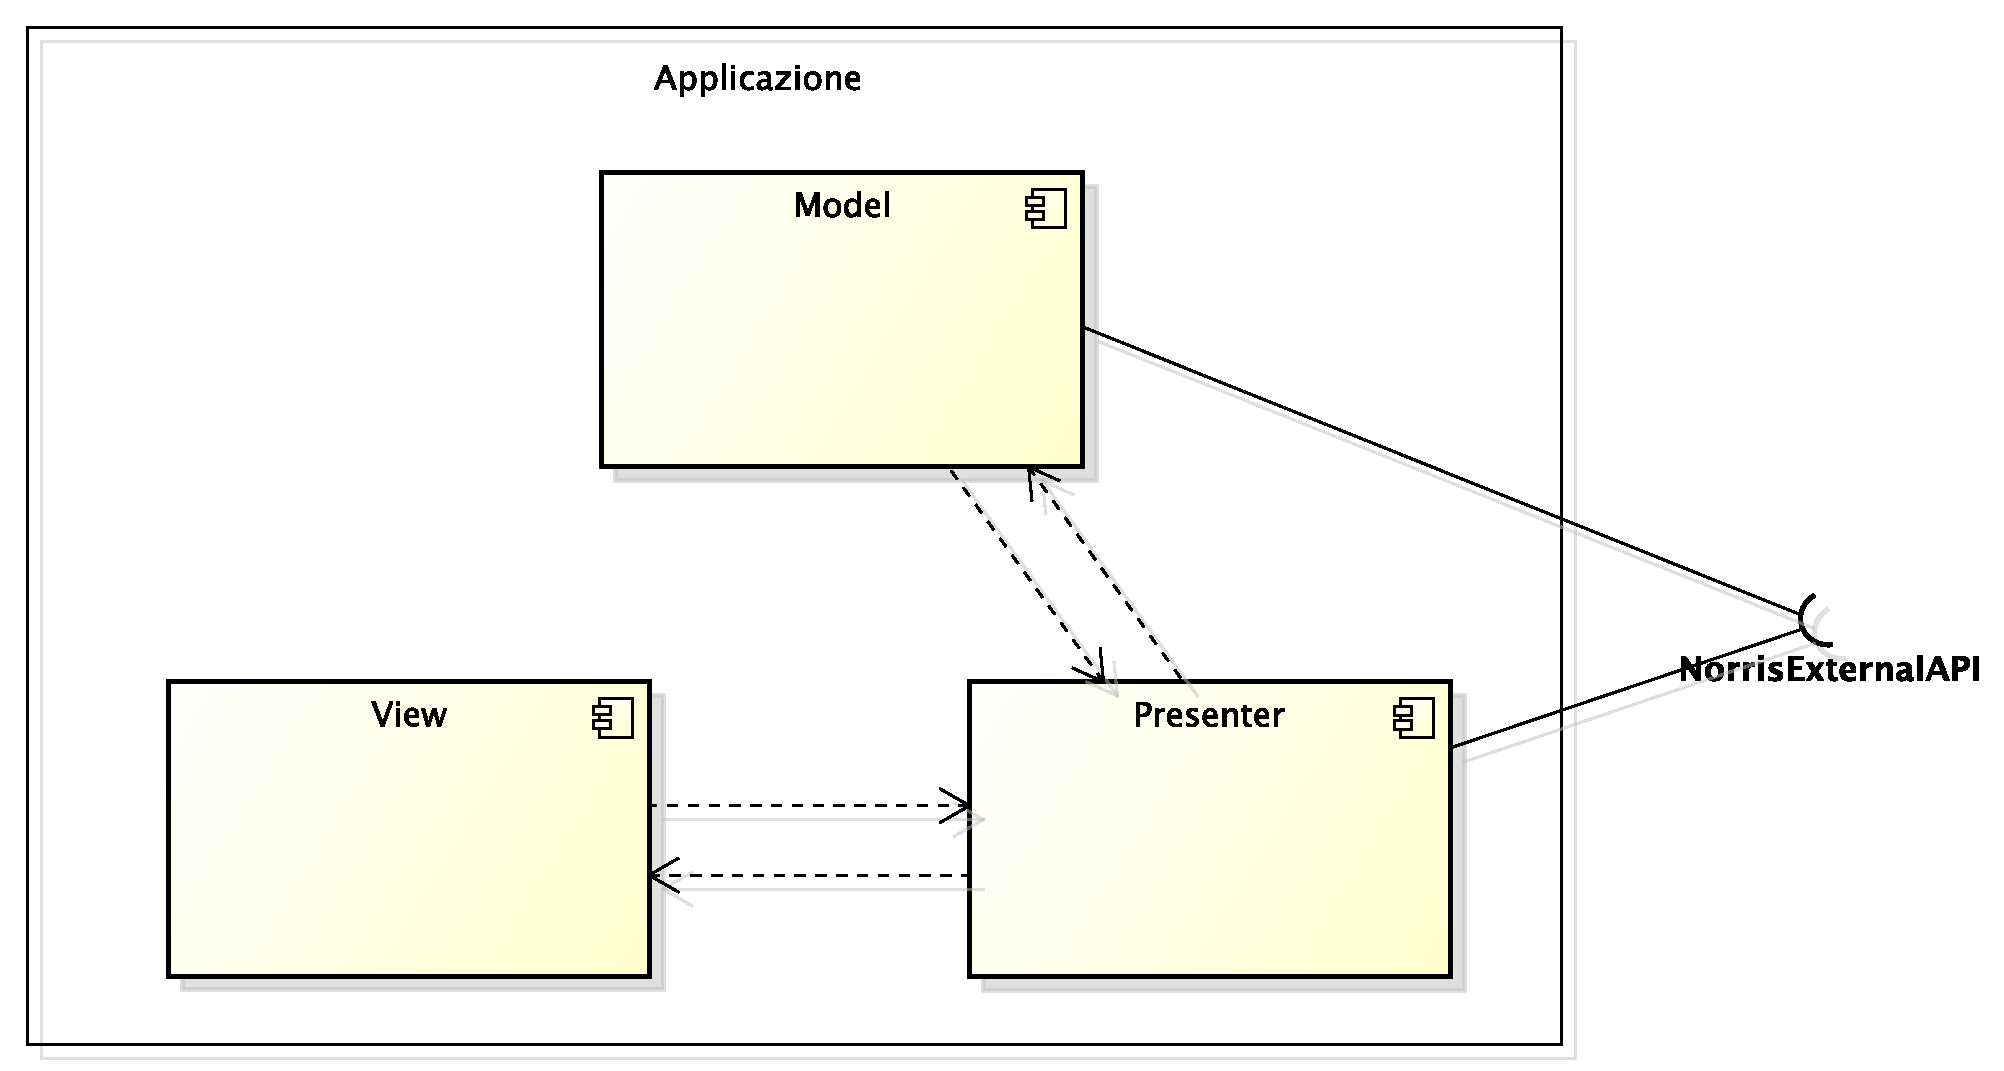
\includegraphics[width=\textwidth]{SpecificaTecnica/Pics/ComponentiApplicazione}
            \caption{Diagramma delle componenti dell'Applicazione Android}
        \end{figure}
        Di seguito vengono descritti i ruoli e le responsabilità delle varie componenti che sono state individuate durante la progettazione architetturale dell'Applicazione Android.
    	\level{4}{Model} 
            Il Model è la componente che rappresenta l'astrazione dei grafici visualizzati nell'applicazione. In essa sono contenuti i dati riguardanti i grafici, assieme alle relative impostazioni. In particolare sono presenti i modelli di tutte le tipologie di chart implementati da \insglo{Norris}. Il Model fornisce per ciascuna tipologia di grafico i metodi per inserire i dati e configurare alcune impostazioni. Si occupa inoltre di gestire gli aggiornamenti dei grafici mantenendo una comunicazione con Norris tramite un canale websocket e di richiedere un chart utilizzando le \insglo{API} esterne di \insglo{Norris}. Infine nel Model sono memorizzate tutte le informazioni inerenti lo stato della sessione con l'istanza di Norris contenente i grafici che si vogliono visualizzare con l'applicazione.
    
       \level{4}{View}
        La View è il componente che rappresenta le varie UI dell'applicazione. In tale componente potrebbero esser sollevati degli eventi scatenati dall'utente attraverso User Gesture. Questi eventi vengono mandati al Presenter che deciderà come comportarsi.
       \level{4}{Presenter}
        Questo componente ha il compito di gestire tutto il controllo dell'applicazione. Le operazioni che esso gestisce sono riassunte nel seguente elenco:
        	\begin{itemize}
        		\item creazione del modello qualora questo sia necessario;
        		\item utilizzo delle \insglo{API} esterne di \insglo{Norris} (Autenticazione, Richiesta della lista);
        		\item interpretazione dei pacchetti ricevuti dal \insglo{server} contenenti i dati delle richieste \insglo{API} effettuate;
                \item chiede al modello di attivare gli aggiornamenti per un certo grafico.
        		\item interpretazione dei pacchetti di aggiornamento;
        		\item richiesta al modello di aggiornare il proprio stato;
        		\item modifica della view;
        		\item avvio delle varie \insglo{activity} dell'applicazione;
        		\item gestione delle \insglo{gesture} dell'utente.
        \end{itemize}
    \level{3}{Descrizione delle interazioni tra le componenti}
    	Le interazioni tra i componenti sono rappresentati con una freccia tratteggiata.\\
    	Riportiamo di seguito la descrizione di ogni interazione.

    	\level{4}{View - Presenter}
        In seguito all'esecuzione di una \insglo{gesture} da parte dell'utente, la View notifica il Presenter tramite l'emissione dell'evento opportuno. Il Presenter si occupa quindi di gestire quest'ultimo. Questa interazione si verifica in particolare quando l'utente seleziona un item della lista dei grafici presenti nell'istanza di \insglo{Norris} richiesta.

        \level{4}{Presenter - View}
        Tale interazione rappresenta la selezione di un'activity modifica tale view. Ciò avviene ad ogni necessità di cambiare \insglo{Activity} e/o quando deve modificare o inizializare la view.

        \level{4}{Presenter - Model}
        Il Presenter richiede al Model di modificare il proprio stato. Ciò avviene per esempio subito dopo l'utilizzo dell'\insglo{API} esterna di \insglo{Norris} per richiedere un grafico o in seguito all'arrivo di un pacchetto di aggiornamento.

        \level{4}{Model - Presenter}
        Tale interazione rappresenta l'invio dei valori del chart provenienti dal server norris oppure, se nel Model è stato attivato il socket per l'aggiornamento, rappresenta la notifica del Model verso il Presenter di avvenuta modifica del chart sul server.
        
		\level{4}{Esempio di interazione tra le componenti}
			\begin{figure}[H]\centering
	        		\includegraphics[width=\textwidth]{SpecificaTecnica/Pics/Model-Presenter}
	        		\caption{Interazione tra Model e Presenter}
	    		\end{figure}
        
    \level{3}{Design pattern utilizzati con le componenti}
    Riportiamo di seguito i pattern architetturali utilizzati nella progettazione delle componenti dell'applicazione Android.
        \level{4}{Model View Presenter}
            Model-View-Presenter (\insglo{MVP}) è un \insglo{pattern} architetturale utilizzato per separare il codice in blocchi di funzionalità ben distinte.\\
            Per la descrizione del \insglo{pattern} e dei vantaggi derivanti dalla sua applicazione si rimanda all'appendice \nameref{app:MVP}.
            \level{5}{Contesto di utilizzo}
                L'\insglo{MVP} viene utilizzato per dividere le classi dell'applicazione \insglo{Android} in tre grandi componenti:
                \begin{itemize}
                    \item Model;
                    \item View;
                    \item Presenter;
                \end{itemize}

    \level{3}{Descrizione delle classi dell'Applicazione Android}
        In questa sezione sono presenti le descrizioni di tutte le classi presenti all'interno del \insglo{prodotto} Applicazione Android. Queste sono state suddivise in base al componente nelle quali sono contenute.
        \level{1}{Applicazione}

	\level{2}{Classi}
		\level{1}{Applicazione}

	\level{2}{Classi}
		\level{1}{Applicazione}

	\level{2}{Classi}
		\input{Classi/Applicazione.tex}
        \level{3}{Classi aggiuntive Applicazione}
	Le interfacce Applicazione::DataModel::DataObject, Applicazione::DataModel::SettingsObject e Applicazione::DataModel::UpdateObject rappresentano genericamente i vari oggetti che utilizzeremo per rappresentare i dati, le impostazioni e gli aggiornamamenti. Tali oggetti sono nel formato JSON ed essendo molto numerosi abbiamo deciso di non inserirle nel diagramma ma di elencarle e descriverle di seguito.

	\begin{itemize}
		\item \textbf{Applicazione::DataModel::BarChartDataObject} Questa classe implementa l'interfaccia Applicazione::DataModel::DataObject. Essa si occupa di rappresentare i dati di un grafico bar chart;

		\item \textbf{Applicazione::DataModel::LineChartDataObject} Questa classe implementa l'interfaccia Applicazione::DataModel::DataObject. Essa si occupa di rappresentare i dati di un grafico line chart;

		\item \textbf{Applicazione::DataModel::MapChartDataObject} Questa classe implementa l'interfaccia Applicazione::DataModel::DataObject. Essa si occupa di rappresentare i dati di un grafico map chart;

		\item \textbf{Applicazione::DataModel::TableDataObject} Questa classe implementa l'interfaccia Applicazione::DataModel::DataObject. Essa si occupa di rappresentare i dati di un grafico table;

		\item \textbf{Applicazione::DataModel::BarChartSettingObject} Questa classe implementa l'interfaccia Applicazione::DataModel::SettingObject. Essa rappresenta le impostazioni di un grafico di tipo bar chart;

		\item \textbf{Applicazione::DataModel::LineChartSettingObject} Questa classe implementa l'interfaccia Applicazione::DataModel::SettingObject. Essa rappresenta le impostazioni di un grafico di tipo line chart;

		\item \textbf{Applicazione::DataModel::MapChartSettingObject} Questa classe implementa l'interfaccia Applicazione::DataModel::SettingObject. Essa rappresenta le impostazioni di un grafico di tipo map chart;

		\item \textbf{Applicazione::DataModel::TableSettingObject} Questa classe implementa l'interfaccia Applicazione::DataModel::SettingObject. Essa rappresenta le impostazioni di un grafico di tipo table;

		\item \textbf{Applicazione::DataModel::BarChartInPlaceUpdateObject} Questa classe implementa l'interfaccia Applicazione::DataModel::UpdateObject. Essa rappresenta un pacchetto di aggiornamento di tipo in place per un grafico di tipo bar chart;

		\item \textbf{Applicazione::DataModel::LineChartInPlaceUpdateObject} Questa classe implementa l'interfaccia Applicazione::DataModel::UpdateObject. Essa rappresenta un pacchetto di aggiornamento di tipo in place per un grafico di tipo line chart;

		\item \textbf{Applicazione::DataModel::LineChartStreamUpdateObject} Questa classe implementa l'interfaccia Applicazione::DataModel::UpdateObject. Essa rappresenta un pacchetto di aggiornamento di tipo stream per un grafico di tipo line chart;

		\item \textbf{Applicazione::DataModel::MapChartInPlaceUpdateObject} Questa classe implementa l'interfaccia Applicazione::DataModel::UpdateObject. Essa rappresenta un pacchetto di aggiornamento di tipo in place per un grafico di tipo map chart;

		\item \textbf{Applicazione::DataModel::MapChartMovieUpdateObject} Questa classe implementa l'interfaccia Applicazione::DataModel::UpdateObject. Essa rappresenta un pacchetto di aggiornamento di tipo movie per un grafico di tipo map chart;

		\item \textbf{Applicazione::DataModel::TableStreamUpdateObject} Questa classe implementa l'interfaccia Applicazione::DataModel::UpdateObject. Essa rappresenta un pacchetto di aggiornamento di tipo stream per un grafico di tipo table;

		\item \textbf{Applicazione::DataModel::TableInPlaceUpdateObject} Questa classe implementa l'interfaccia Applicazione::DataModel::UpdateObject. Essa rappresenta un pacchetto di aggiornamento di tipo in place per un grafico di tipo table.
	\end{itemize}
    \level{3}{Interazioni tra classi dei componenti dell'applicazione Android}
	Dopo che sono stati descritte nel dettaglio tutte le varie classi necessarie alla progettazione dell'applicazione \insglo{Android}, è necessario mostrare come le classi appartenenti a componenti differenti interagiscano tra di loro. È quindi inserito in seguito un diagramma \insglo{UML} che rappresenta tutte le interazioni presenti tra i vari componenti.\\
	Si noti che alcune classi non sono state inserite in quanto si è voluto rendere più comprensibile il diagramma.

	\begin{figure}[H]\centering
		\includegraphics[width=\textwidth]{SpecificaTecnica/Pics/InterazioniComponentiApplicazione.pdf}
		\caption{Diagramma delle interazioni tra classi di componenti dell'Applicazione}
	\end{figure}

    \level{3}{Design pattern utilizzati con le classi}
        Nella progettazione delle classi dell'applicazione abbiamo deciso di utilizzare alcuni \insglo{design pattern}. Riportiamo di seguito una loro breve descrizione e il contesto nel quale sono stati utilizzati.
        
        \level{4}{Adapter}
            Il \insglo{pattern} strutturale Adapter viene utilizzato per adattare l'interfaccia di una classe in un'altra.\\
            Per la descrizione del \insglo{pattern} e dei vantaggi derivanti dalla sua applicazione si rimanda all'appendice \nameref{app:adapter}.
            \level{5}{Contesto di utilizzo}
                Nell'applicazione \insglo{Android} l'Adapter viene utilizzato per calare le varie librerie esterne nel contesto di \projectname{}, e nello specifico sono rappresentate dalle diverse View, quindi:
                \begin{itemize}
                    \item View::BarChartActivity è un adattatore per MPABarChart;
                    \item View::MapChartActivity è un adattatore per GoogleMap \insglo{Android} \insglo{API} v2;
                    \item View::LineChartActivity è un adattatore per MPALineChart.
                \end{itemize}
                
        \level{4}{Dependency Injection}
            Dependency Injection è un \insglo{pattern} architetturale il cui scopo è separare il comportamento di una componente dalla risoluzione delle sue dipendenze.\\
            Per la descrizione del \insglo{pattern} e dei vantaggi derivanti dalla sua applicazione si rimanda all'appendice \nameref{app:dependencyinjection}.
            \level{5}{Contesto di utilizzo}
                La Dependency Injection viene utilizzata con le classi che implementano le seguenti interfacce:
                \begin{itemize}
                    \item Model::NorrisChart::ChartFactory, inietta in Model::NorrisChart::ChartImpl le  corrispondenze tra i tipi di grafico e le rispettive classi factory;
                    \item Model::NorrisChart::Updater, inietta in Model::NorrisChart::ChartImpl le corrispondenze tra i diversi tipi di aggiornamenti e le classi che li implementano;
                     \item Presenter::PresenterFactory, inietta in Presenter::PresenterImpl le corrispondenze tra i tipi di presenter e le rispettive classi factory.
                    \begin{figure}[H]\centering
	        		\includegraphics[width=\textwidth]{SpecificaTecnica/Pics/DesignPatternNorris/DependencyInjection2}
	        		\caption{Dependency Injection pattern nell'applicazione Android}
	    		\end{figure}
	    		\begin{figure}[H]\centering
	        		\includegraphics[width=\textwidth]{SpecificaTecnica/Pics/DesignPatternNorris/DependencyInjection1}
	        		\caption{Dependency Injection pattern nell'applicazione Android}
	    		\end{figure}
                \end{itemize}
                
         \level{4}{Factory Method}
            Il \insglo{pattern} creazionale Factory Method si occupa di fornire un'interfaccia per la creazione di famiglie di prodotti, senza dover specificare classi concrete. \\
            Per la descrizione del \insglo{pattern} e dei vantaggi derivanti dalla sua applicazione si rimanda all'appendice \nameref{app:factorymethod}.
            \level{5}{Contesto di utilizzo}
                Gli elementi che implementano Factory Method sono:
                \begin{itemize}
                \item Interfacce:
                    \begin{itemize}
                        \item Model::NorrisChart::ChartFactory, con cui vengono generati i diversi tipi di grafici;
                        \item Presenter::PresenterFactory, con cui sono generati i diversi tipi di presenter dei grafici.
                    \end{itemize}
                \item Classi:
                    \begin{itemize}
                        \item Model::NorrisChart::BarChartFactory;
                        \item Model::NorrisChart::LineChartFactory;
                        \item Model::NorrisChart::MapChartFactory;
                        \item Model::NorrisChart::TableFactory;
                        \item Presenter::BarChartPresenterFactory;
                        \item Presenter::LineChartPresenterFactory;
                        \item Presenter::MapChartPresenterFactory;
                        \item Presenter::TablePresenterFactory;
                        \item Presenter::ListPresenterFactory;
                        \item Presenter::LoginPresenterFactory.
                    \end{itemize}
                \end{itemize}
                \begin{figure}[H]\centering
	        		\includegraphics[width=\textwidth]{SpecificaTecnica/Pics/DesignPatternNorris/Factory2}
	        		\caption{Factory Method pattern nell'applicazione Android}
	    		\end{figure}

                
        \level{4}{Observer}
            L'Observer è un \insglo{pattern} comportamentale che ha lo scopo di monitorare lo stato di diversi oggetti legati ad un soggetto. Per la descrizione del \insglo{pattern} e dei vantaggi derivanti dalla sua applicazione si rimanda all'appendice \nameref{app:observer}.
            \level{5}{Contesto di utilizzo}
                % Il \insglo{pattern} Observer si basa sugli oggetti “osservabili” e sugli “osservatori”. \\ Nell'applicazione \insglo{Android} il nucleo dell'implementazione dell'Observer si trova nel \insglo{package} Utils, in cui sono contenute le interfacce Utils::Observer e Utils::Observable, e la classe Utils::ObservableImpl (implementazione di Utils::Observable). Questi tre elementi vengono poi estesi o implementati dagli altri elementi della libreria per realizzare il \insglo{pattern} completo.\\
                Classi che implementano Observer:
                \begin{itemize}
                    \item Presenter::ChartPresenterImpl;
                \end{itemize}
                Classi che estendono Observable:
                \begin{itemize}
                    \item Model::Service::ChartReceiverImpl.
                \end{itemize}
                
        \level{4}{Singleton}
            Il Singleton è un \insglo{pattern} creazionale il cui scopo è permettere la creazione di una sola istanza di una classe, nonchè di fornire un punto di accesso globale ad essa.\\
            Per la descrizione del \insglo{pattern} e dei vantaggi derivanti dalla sua applicazione si rimanda all'appendice \nameref{app:singleton}.
            \level{5}{Contesto di utilizzo}
                Nell'applicazione \insglo{Android} il Singleton viene implementato nelle seguenti classi:
                \begin{itemize}
                        \item Model::NorrisChart::BarChartFactory;
                        \item Model::NorrisChart::LineChartFactory;
                        \item Model::NorrisChart::MapChartFactory;
                        \item Model::NorrisChart::TableFactory;
                        \item Model::NorrisChart::BarChartInPlaceUpdater;
						\item Model::NorrisChart::LineChartInPlaceUpdater;
						\item Model::NorrisChart::LineChartStreamUpdater;
						\item Model::NorrisChart::MapChartInPlaceUpdater;
						\item Model::NorrisChart::MapChartMovieUpdater;
						\item Model::NorrisChart::TableInPlaceUpdater;
						\item Model::NorrisChart::TableStreamUpdater
                        \item Model::Service::ChartReceiverImpl;
                        \item Model::NorrisSessionInfoImpl;
                        \item Presenter::BarChartPresenterFactory;
                        \item Presenter::LineChartPresenterFactory;
                        \item Presenter::MapChartPresenterFactory;
                        \item Presenter::TablePresenterFactory;
                        \item Presenter::ListPresenterFactory;
                        \item Presenter::LoginPresenterFactory;
                        \item Presenter::JSONParser.
                    \end{itemize}
                    \begin{figure}[H]\centering
	        		\includegraphics[width=\textwidth]{SpecificaTecnica/Pics/DesignPatternNorris/Singleton2}
	        		\caption{Singleton pattern nell'applicazione Android}
	    		\end{figure}
	    		\begin{figure}[H]\centering
	        		\includegraphics[width=\textwidth]{SpecificaTecnica/Pics/DesignPatternNorris/Singleton1}
	        		\caption{Singleton pattern nell'applicazione Android}
	    		\end{figure}
	    		\level{4}{Strategy}
			Strategy è un design pattern comportamentale che offre la possibilità di definire una famiglia di
algoritmi, incapsularli e renderli intercambiabili. Per la descrizione del \insglo{pattern} e dei vantaggi derivanti dalla sua applicazione si rimanda all'appendice \nameref{app:strategy}.
				\level{5}{Contesto di utilizzo}
					Le classi che implementano lo Strategy sono quelle che si occupano di aggiornare i diversi tipi di grafici. Le riportiamo di seguito:
					\begin{itemize}
					\item Model::NorrisChart::BarChartInPlaceUpdater;
					\item Model::NorrisChart::LineChartInPlaceUpdater;
					\item Model::NorrisChart::LineChartStreamUpdater;
					\item Model::NorrisChart::MapChartInPlaceUpdater;
					\item Model::NorrisChart::MapChartMovieUpdater;
					\item Model::NorrisChart::TableInPlaceUpdater;
					\item Model::NorrisChart::TableStreamUpdater.
				\end{itemize}
				\begin{figure}[H]\centering
	        		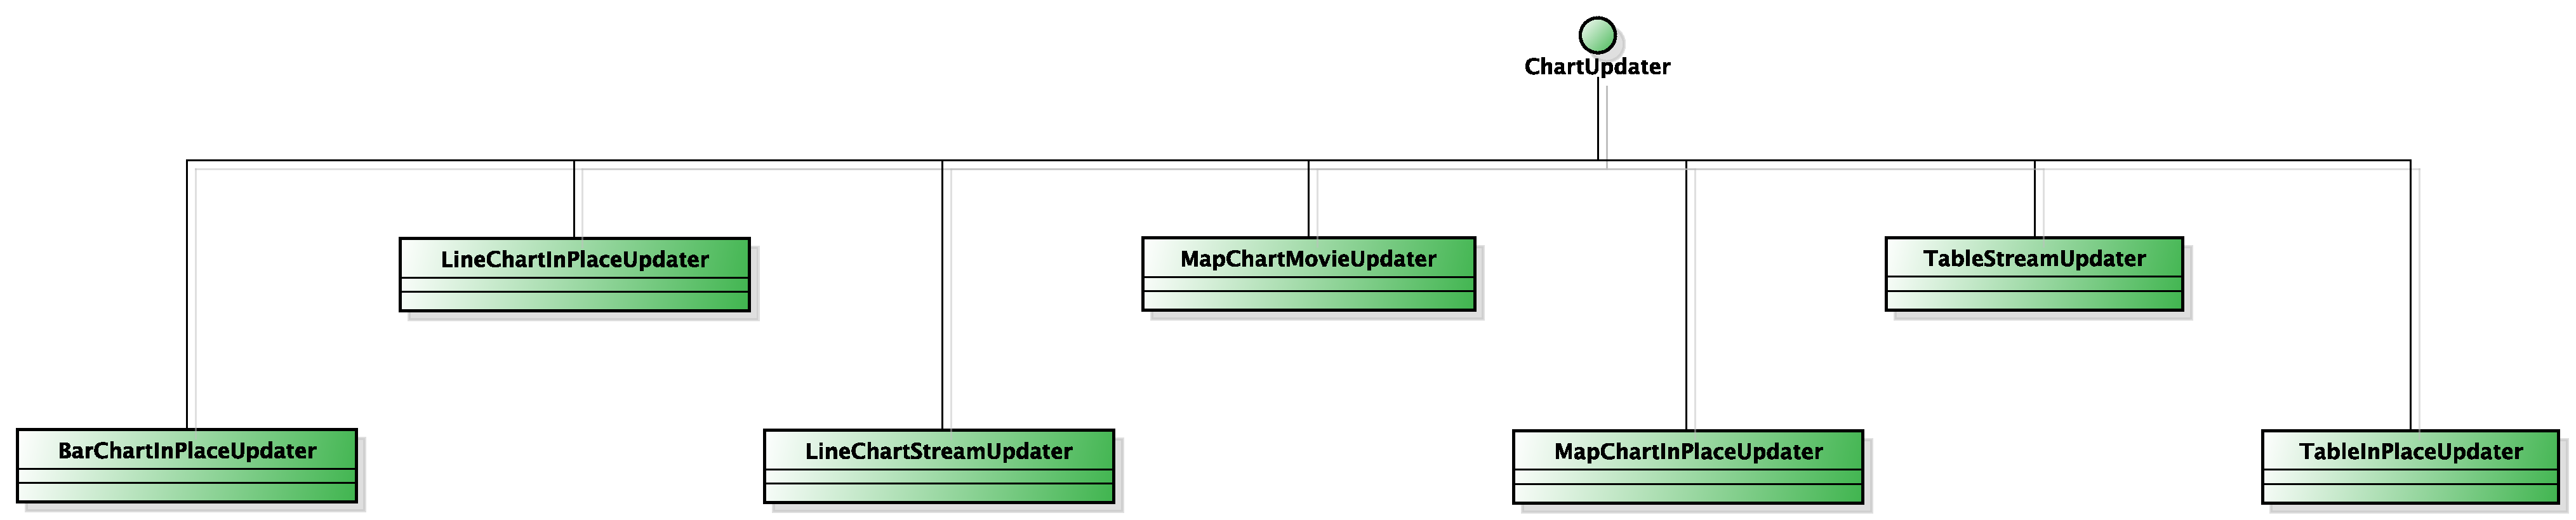
\includegraphics[width=\textwidth]{SpecificaTecnica/Pics/DesignPatternNorris/Strategy}
	        		\caption{Strategy pattern nell'applicazione Android}
	    		\end{figure}

